\documentclass{article}
\usepackage{tikz}
\usepackage{xcolor}


\begin{document}
	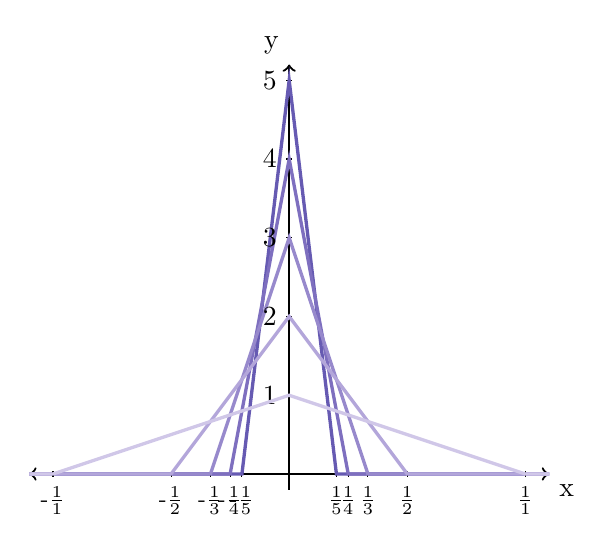
\begin{tikzpicture}
		%GRADIENTE
		\definecolor{myblue}{cmyk}{90,80,0,0}

		%EJES
		\draw[thick,<->] (-3.3,0) -- (3.3,0) node[anchor=north west] {x};
		\draw[thick,->] (0,-0.2) -- (0,5.2) node[anchor=south east] {y};
		
		%BUCLE FUNCIONES
		\foreach \x in {5,...,1}{
			%ETIQUETAS
			\draw ({3/(\x)},1pt) -- ({3/(\x)},-1pt) node[anchor=north] {\footnotesize$\frac{1}{\x}$};
			\draw (-{3/(\x)},1pt) -- (-{3/(\x)},-1pt) node[anchor=north] {\footnotesize-$\frac{1}{\x}$};
			\draw (1pt,\x cm) -- (-1pt,\x cm) node[anchor=east] {$\x$};
			%GRADIENTE
			\pgfmathsetmacro\k{\x*12+6}
			%FUNCION
			\draw[color=myblue!\k, very thick] (-3.3,0) -- ({-3/(\x)},0) -- (0,\x) -- ({3/(\x)},0) -- (3.3,0);
		}
	\end{tikzpicture}
\end{document}